\newpage
\section{Introduction}
\label{sec:introduction}

% state the learning objective 
In this lab assignment, we will be presenting a circuit made by us, including an envelope detector and a voltage regulator, as well as a transformer and a voltage source.

The envolpe detector is made up by a voltage source, fours diodes, a resistance and a capacitor, with the diodes being displayed in a diamond shape, so the current goes through one of the pairs of diodes, one being having the positive current and another the negative.

The voltage regulator is made up of a voltage source, a resistance, and a varying number of diodes in series. In our case, we have 20 diodes.

The circuit above described is displayed in Figure \ref{fig:circuit}.

\begin{figure}[h] \centering
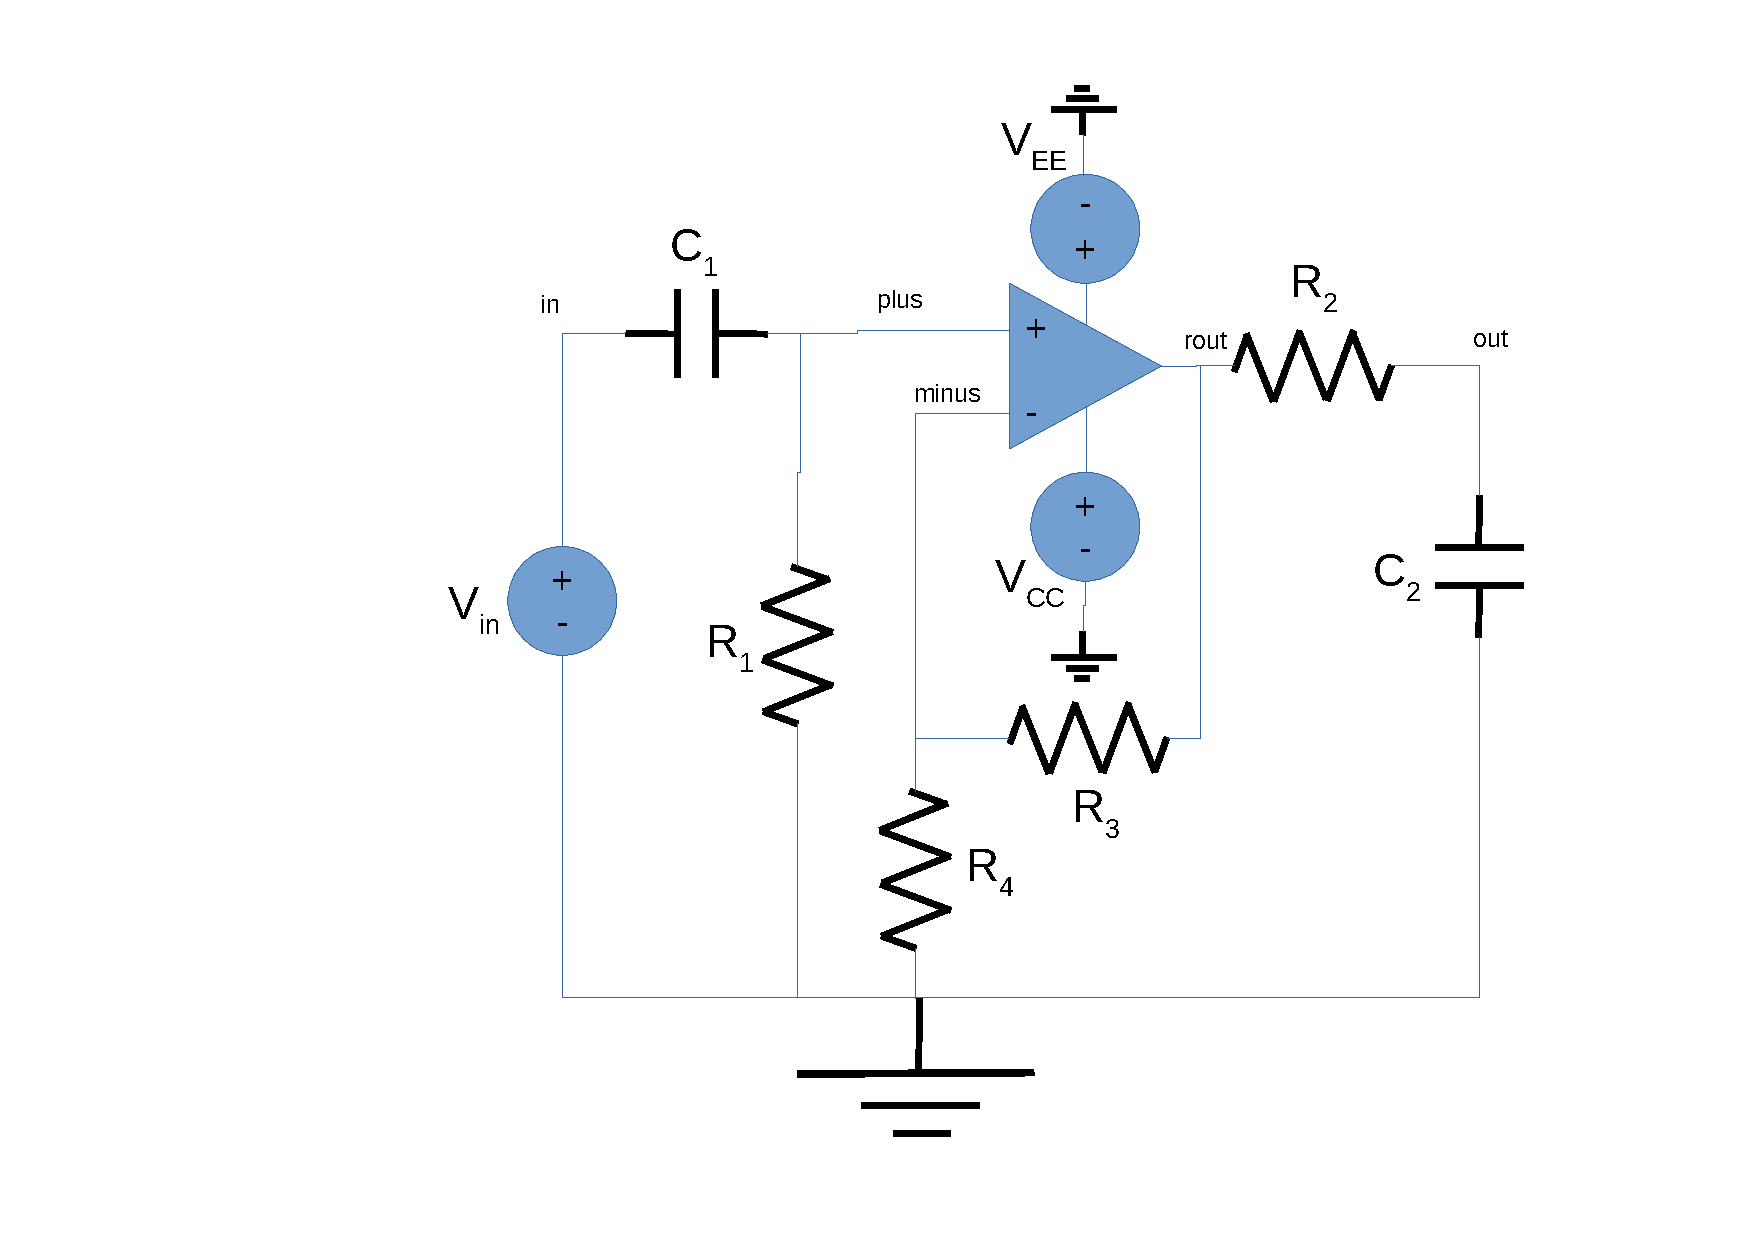
\includegraphics[width=0.6\linewidth]{circuit.pdf}
\caption{The circuit we will be working with.}
\label{fig:circuit}
\end{figure}

Considering this assignment strongly relies on diodes and how they work, it makes sense to explain it.

\begin{figure}[h] \centering
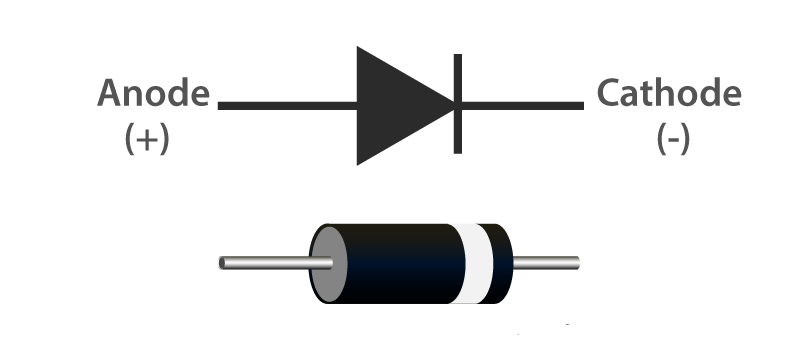
\includegraphics[width=0.6\linewidth]{Diodes-symbol.png}
\caption{Diode Scheme \cite{diode-image}}
\label{fig:diode}
\end{figure}

In Section~\ref{sec:analysis}, a theoretical analysis of the circuit is
presented, including an individual analysis for the envelope detector and the voltage regulator.
In Section~\ref{sec:simulation}, the circuit is analysed by
simulation using the \textit{software Ngspice}, ultimately, studying the same as in the Theoretical Analysis section.
The results in each Analsysis are compared \ref{sec:comparing}.
The conclusions of this study are outlined in
Section~\ref{sec:conclusion}.
